% Options for packages loaded elsewhere
\PassOptionsToPackage{unicode}{hyperref}
\PassOptionsToPackage{hyphens}{url}
%
\documentclass[
]{article}
\usepackage{amsmath,amssymb}
\usepackage{iftex}
\ifPDFTeX
  \usepackage[T1]{fontenc}
  \usepackage[utf8]{inputenc}
  \usepackage{textcomp} % provide euro and other symbols
\else % if luatex or xetex
  \usepackage{unicode-math} % this also loads fontspec
  \defaultfontfeatures{Scale=MatchLowercase}
  \defaultfontfeatures[\rmfamily]{Ligatures=TeX,Scale=1}
\fi
\usepackage{lmodern}
\ifPDFTeX\else
  % xetex/luatex font selection
\fi
% Use upquote if available, for straight quotes in verbatim environments
\IfFileExists{upquote.sty}{\usepackage{upquote}}{}
\IfFileExists{microtype.sty}{% use microtype if available
  \usepackage[]{microtype}
  \UseMicrotypeSet[protrusion]{basicmath} % disable protrusion for tt fonts
}{}
\makeatletter
\@ifundefined{KOMAClassName}{% if non-KOMA class
  \IfFileExists{parskip.sty}{%
    \usepackage{parskip}
  }{% else
    \setlength{\parindent}{0pt}
    \setlength{\parskip}{6pt plus 2pt minus 1pt}}
}{% if KOMA class
  \KOMAoptions{parskip=half}}
\makeatother
\usepackage{xcolor}
\usepackage[margin=1in]{geometry}
\usepackage{color}
\usepackage{fancyvrb}
\newcommand{\VerbBar}{|}
\newcommand{\VERB}{\Verb[commandchars=\\\{\}]}
\DefineVerbatimEnvironment{Highlighting}{Verbatim}{commandchars=\\\{\}}
% Add ',fontsize=\small' for more characters per line
\usepackage{framed}
\definecolor{shadecolor}{RGB}{248,248,248}
\newenvironment{Shaded}{\begin{snugshade}}{\end{snugshade}}
\newcommand{\AlertTok}[1]{\textcolor[rgb]{0.94,0.16,0.16}{#1}}
\newcommand{\AnnotationTok}[1]{\textcolor[rgb]{0.56,0.35,0.01}{\textbf{\textit{#1}}}}
\newcommand{\AttributeTok}[1]{\textcolor[rgb]{0.13,0.29,0.53}{#1}}
\newcommand{\BaseNTok}[1]{\textcolor[rgb]{0.00,0.00,0.81}{#1}}
\newcommand{\BuiltInTok}[1]{#1}
\newcommand{\CharTok}[1]{\textcolor[rgb]{0.31,0.60,0.02}{#1}}
\newcommand{\CommentTok}[1]{\textcolor[rgb]{0.56,0.35,0.01}{\textit{#1}}}
\newcommand{\CommentVarTok}[1]{\textcolor[rgb]{0.56,0.35,0.01}{\textbf{\textit{#1}}}}
\newcommand{\ConstantTok}[1]{\textcolor[rgb]{0.56,0.35,0.01}{#1}}
\newcommand{\ControlFlowTok}[1]{\textcolor[rgb]{0.13,0.29,0.53}{\textbf{#1}}}
\newcommand{\DataTypeTok}[1]{\textcolor[rgb]{0.13,0.29,0.53}{#1}}
\newcommand{\DecValTok}[1]{\textcolor[rgb]{0.00,0.00,0.81}{#1}}
\newcommand{\DocumentationTok}[1]{\textcolor[rgb]{0.56,0.35,0.01}{\textbf{\textit{#1}}}}
\newcommand{\ErrorTok}[1]{\textcolor[rgb]{0.64,0.00,0.00}{\textbf{#1}}}
\newcommand{\ExtensionTok}[1]{#1}
\newcommand{\FloatTok}[1]{\textcolor[rgb]{0.00,0.00,0.81}{#1}}
\newcommand{\FunctionTok}[1]{\textcolor[rgb]{0.13,0.29,0.53}{\textbf{#1}}}
\newcommand{\ImportTok}[1]{#1}
\newcommand{\InformationTok}[1]{\textcolor[rgb]{0.56,0.35,0.01}{\textbf{\textit{#1}}}}
\newcommand{\KeywordTok}[1]{\textcolor[rgb]{0.13,0.29,0.53}{\textbf{#1}}}
\newcommand{\NormalTok}[1]{#1}
\newcommand{\OperatorTok}[1]{\textcolor[rgb]{0.81,0.36,0.00}{\textbf{#1}}}
\newcommand{\OtherTok}[1]{\textcolor[rgb]{0.56,0.35,0.01}{#1}}
\newcommand{\PreprocessorTok}[1]{\textcolor[rgb]{0.56,0.35,0.01}{\textit{#1}}}
\newcommand{\RegionMarkerTok}[1]{#1}
\newcommand{\SpecialCharTok}[1]{\textcolor[rgb]{0.81,0.36,0.00}{\textbf{#1}}}
\newcommand{\SpecialStringTok}[1]{\textcolor[rgb]{0.31,0.60,0.02}{#1}}
\newcommand{\StringTok}[1]{\textcolor[rgb]{0.31,0.60,0.02}{#1}}
\newcommand{\VariableTok}[1]{\textcolor[rgb]{0.00,0.00,0.00}{#1}}
\newcommand{\VerbatimStringTok}[1]{\textcolor[rgb]{0.31,0.60,0.02}{#1}}
\newcommand{\WarningTok}[1]{\textcolor[rgb]{0.56,0.35,0.01}{\textbf{\textit{#1}}}}
\usepackage{graphicx}
\makeatletter
\def\maxwidth{\ifdim\Gin@nat@width>\linewidth\linewidth\else\Gin@nat@width\fi}
\def\maxheight{\ifdim\Gin@nat@height>\textheight\textheight\else\Gin@nat@height\fi}
\makeatother
% Scale images if necessary, so that they will not overflow the page
% margins by default, and it is still possible to overwrite the defaults
% using explicit options in \includegraphics[width, height, ...]{}
\setkeys{Gin}{width=\maxwidth,height=\maxheight,keepaspectratio}
% Set default figure placement to htbp
\makeatletter
\def\fps@figure{htbp}
\makeatother
\setlength{\emergencystretch}{3em} % prevent overfull lines
\providecommand{\tightlist}{%
  \setlength{\itemsep}{0pt}\setlength{\parskip}{0pt}}
\setcounter{secnumdepth}{-\maxdimen} % remove section numbering
\ifLuaTeX
  \usepackage{selnolig}  % disable illegal ligatures
\fi
\IfFileExists{bookmark.sty}{\usepackage{bookmark}}{\usepackage{hyperref}}
\IfFileExists{xurl.sty}{\usepackage{xurl}}{} % add URL line breaks if available
\urlstyle{same}
\hypersetup{
  pdftitle={REM for Low Performing Sessions},
  hidelinks,
  pdfcreator={LaTeX via pandoc}}

\title{REM for Low Performing Sessions}
\author{}
\date{\vspace{-2.5em}}

\begin{document}
\maketitle

\begin{Shaded}
\begin{Highlighting}[]
\CommentTok{\# Interactions Data Frame (Edges)}
\NormalTok{low\_perf\_interactions }\OtherTok{\textless{}{-}} \FunctionTok{readRDS}\NormalTok{(}\StringTok{"data/low\_performance\_sessions.RData"}\NormalTok{) }\SpecialCharTok{\%\textgreater{}\%} 
  \FunctionTok{select}\NormalTok{(session, sender\_id, receiver\_id, dialog, time)}


\NormalTok{interactions }\OtherTok{\textless{}{-}}\NormalTok{ low\_perf\_interactions }\SpecialCharTok{\%\textgreater{}\%}
  \FunctionTok{mutate}\NormalTok{(}
    \AttributeTok{sender\_id =} \FunctionTok{as.integer}\NormalTok{(sender\_id),  }
    \AttributeTok{receiver\_id =} \FunctionTok{as.integer}\NormalTok{(receiver\_id), }
    \AttributeTok{dialog =} \FunctionTok{as.factor}\NormalTok{(dialog) }
\NormalTok{  )}



\NormalTok{actors\_attributes }\OtherTok{\textless{}{-}} \FunctionTok{data.frame}\NormalTok{(}
  \AttributeTok{id =} \DecValTok{1}\SpecialCharTok{:}\DecValTok{8}\NormalTok{,}
  \AttributeTok{name =} \FunctionTok{c}\NormalTok{(}\StringTok{"Igor"}\NormalTok{, }\StringTok{"Ashley"}\NormalTok{, }\StringTok{"Will"}\NormalTok{, }\StringTok{"Katya"}\NormalTok{, }\StringTok{"Saleh"}\NormalTok{, }\StringTok{"Oleg"}\NormalTok{, }\StringTok{"Vika"}\NormalTok{, }\StringTok{"Alex"}\NormalTok{),}
  \AttributeTok{gender =} \FunctionTok{c}\NormalTok{(}\StringTok{"male"}\NormalTok{, }\StringTok{"female"}\NormalTok{, }\StringTok{"male"}\NormalTok{, }\StringTok{"female"}\NormalTok{, }\StringTok{"male"}\NormalTok{, }\StringTok{"male"}\NormalTok{, }\StringTok{"female"}\NormalTok{, }\StringTok{"male"}\NormalTok{)}
\NormalTok{)}

\CommentTok{\# Create dummy variables for gender}
\NormalTok{dummyvars }\OtherTok{\textless{}{-}} \FunctionTok{dummyVars}\NormalTok{(}\StringTok{" \textasciitilde{} gender"}\NormalTok{, }\AttributeTok{data =}\NormalTok{ actors\_attributes)}
\NormalTok{actors\_attributes }\OtherTok{\textless{}{-}} \FunctionTok{cbind}\NormalTok{(actors\_attributes, }\FunctionTok{predict}\NormalTok{(dummyvars, actors\_attributes)) }\SpecialCharTok{\%\textgreater{}\%}
  \FunctionTok{select}\NormalTok{(id, name, gendermale)}
\end{Highlighting}
\end{Shaded}

\hypertarget{summary-by-session-and-speaker}{%
\subsection{Summary by Session and
Speaker}\label{summary-by-session-and-speaker}}

\begin{Shaded}
\begin{Highlighting}[]
\NormalTok{session\_dialogues }\OtherTok{\textless{}{-}}\NormalTok{ low\_perf\_interactions }\SpecialCharTok{\%\textgreater{}\%}
  \FunctionTok{group\_by}\NormalTok{(session) }\SpecialCharTok{\%\textgreater{}\%}
  \FunctionTok{summarise}\NormalTok{(}\AttributeTok{n =} \FunctionTok{n}\NormalTok{())}


\FunctionTok{ggplot}\NormalTok{(session\_dialogues, }\FunctionTok{aes}\NormalTok{(}\AttributeTok{x =} \FunctionTok{factor}\NormalTok{(session), }\AttributeTok{y =}\NormalTok{ n, }\AttributeTok{fill =} \FunctionTok{factor}\NormalTok{(session))) }\SpecialCharTok{+} 
  \FunctionTok{geom\_bar}\NormalTok{(}\AttributeTok{stat =} \StringTok{"identity"}\NormalTok{) }\SpecialCharTok{+}
  \FunctionTok{scale\_fill\_brewer}\NormalTok{(}\AttributeTok{palette =} \StringTok{"Pastel1"}\NormalTok{) }\SpecialCharTok{+}  
  \FunctionTok{labs}\NormalTok{(}\AttributeTok{title =} \StringTok{"Number of Dialogues Per Session (High Performance)"}\NormalTok{,}
       \AttributeTok{x =} \StringTok{"Session"}\NormalTok{,}
       \AttributeTok{y =} \StringTok{"Number of Dialogues"}\NormalTok{,}
       \AttributeTok{fill =} \StringTok{"Session"}\NormalTok{) }\SpecialCharTok{+}
  \FunctionTok{theme\_minimal}\NormalTok{() }\SpecialCharTok{+} 
  \FunctionTok{theme}\NormalTok{(}\AttributeTok{legend.position =} \StringTok{"none"}\NormalTok{) }
\end{Highlighting}
\end{Shaded}

\begin{center}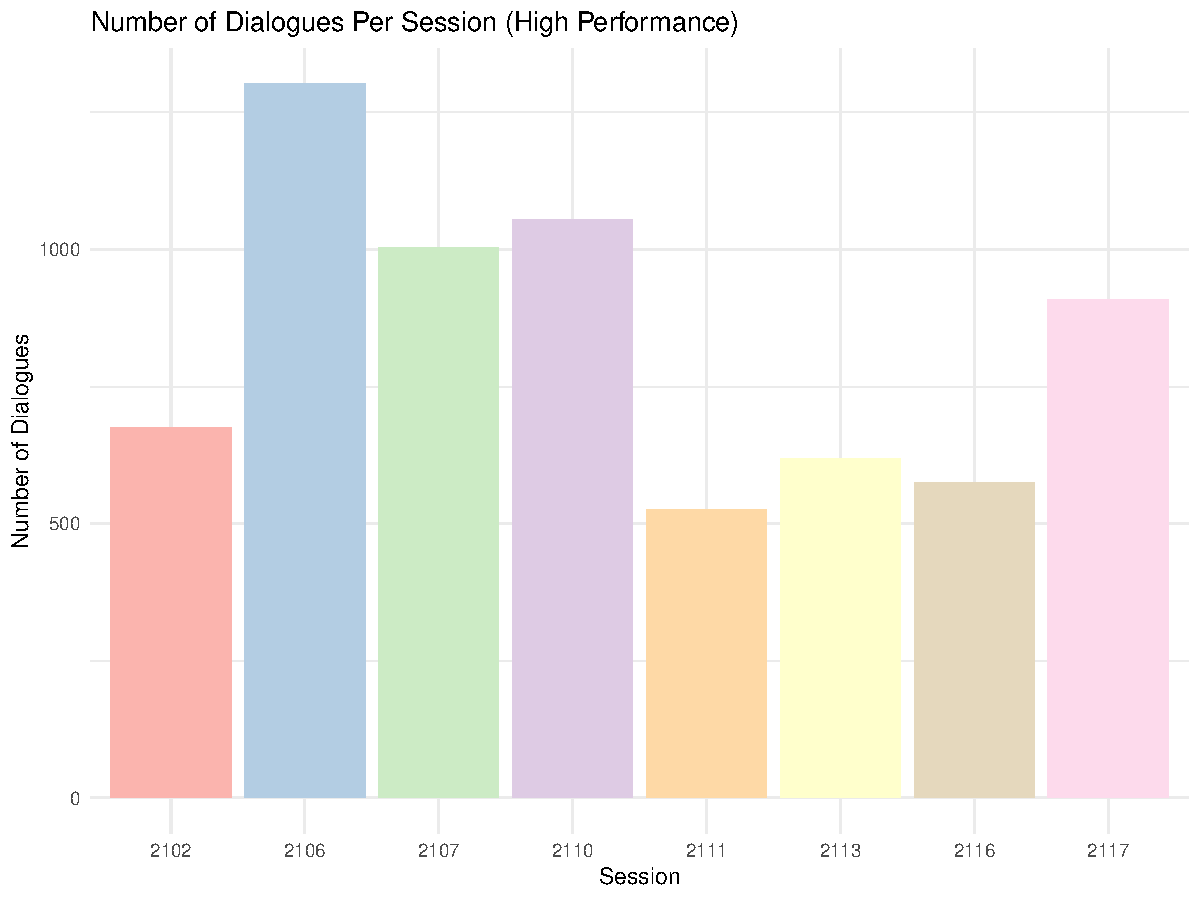
\includegraphics{low_surv_analysis_files/figure-latex/unnamed-chunk-2-1} \end{center}

\begin{Shaded}
\begin{Highlighting}[]
\NormalTok{dialogues\_per\_speaker\_session }\OtherTok{\textless{}{-}}\NormalTok{ low\_perf\_interactions }\SpecialCharTok{\%\textgreater{}\%}
  \FunctionTok{left\_join}\NormalTok{(actors\_attributes, }\AttributeTok{by =} \FunctionTok{c}\NormalTok{(}\StringTok{"sender\_id"} \OtherTok{=} \StringTok{"id"}\NormalTok{)) }\SpecialCharTok{\%\textgreater{}\%}
  \FunctionTok{group\_by}\NormalTok{(session, name) }\SpecialCharTok{\%\textgreater{}\%}
  \FunctionTok{summarise}\NormalTok{(}\AttributeTok{number\_of\_dialogues =} \FunctionTok{n}\NormalTok{(), }\AttributeTok{.groups =} \StringTok{\textquotesingle{}drop\textquotesingle{}}\NormalTok{) }\SpecialCharTok{\%\textgreater{}\%}
  \FunctionTok{arrange}\NormalTok{(session, }\FunctionTok{desc}\NormalTok{(number\_of\_dialogues))}

\NormalTok{dialogues\_summary\_tibble }\OtherTok{\textless{}{-}} \FunctionTok{as\_tibble}\NormalTok{(dialogues\_per\_speaker\_session)}
\FunctionTok{print}\NormalTok{(dialogues\_summary\_tibble)}
\end{Highlighting}
\end{Shaded}

\begin{verbatim}
## # A tibble: 43 x 3
##    session name   number_of_dialogues
##      <dbl> <chr>                <int>
##  1    2102 Igor                   167
##  2    2102 Will                   134
##  3    2102 Oleg                   102
##  4    2102 Vika                    91
##  5    2102 Ashley                  73
##  6    2102 Saleh                   64
##  7    2102 Katya                   44
##  8    2106 Ashley                 389
##  9    2106 Oleg                   292
## 10    2106 Will                   239
## # i 33 more rows
\end{verbatim}

\begin{Shaded}
\begin{Highlighting}[]
\FunctionTok{ggplot}\NormalTok{(dialogues\_summary\_tibble, }\FunctionTok{aes}\NormalTok{(}\AttributeTok{x =}\NormalTok{ name, }\AttributeTok{y =}\NormalTok{ number\_of\_dialogues, }\AttributeTok{fill =}\NormalTok{ name)) }\SpecialCharTok{+} 
  \FunctionTok{geom\_bar}\NormalTok{(}\AttributeTok{stat =} \StringTok{"identity"}\NormalTok{) }\SpecialCharTok{+}
  \FunctionTok{facet\_wrap}\NormalTok{(}\SpecialCharTok{\textasciitilde{}}\NormalTok{session) }\SpecialCharTok{+}
  \FunctionTok{scale\_fill\_brewer}\NormalTok{(}\AttributeTok{palette =} \StringTok{"Pastel1"}\NormalTok{) }\SpecialCharTok{+}  
  \FunctionTok{labs}\NormalTok{(}\AttributeTok{subtitle =} \StringTok{"Number of Dialogues Per Speaker Per Session (High Performance)"}\NormalTok{,}
       \AttributeTok{x =} \StringTok{"Speaker"}\NormalTok{,}
       \AttributeTok{y =} \StringTok{"Number of Dialogues"}\NormalTok{,}
       \AttributeTok{fill =} \StringTok{"Speaker"}\NormalTok{) }\SpecialCharTok{+}
  \FunctionTok{theme\_minimal}\NormalTok{() }\SpecialCharTok{+} 
  \FunctionTok{theme}\NormalTok{(}\AttributeTok{legend.position =} \StringTok{"none"}\NormalTok{) }
\end{Highlighting}
\end{Shaded}

\begin{center}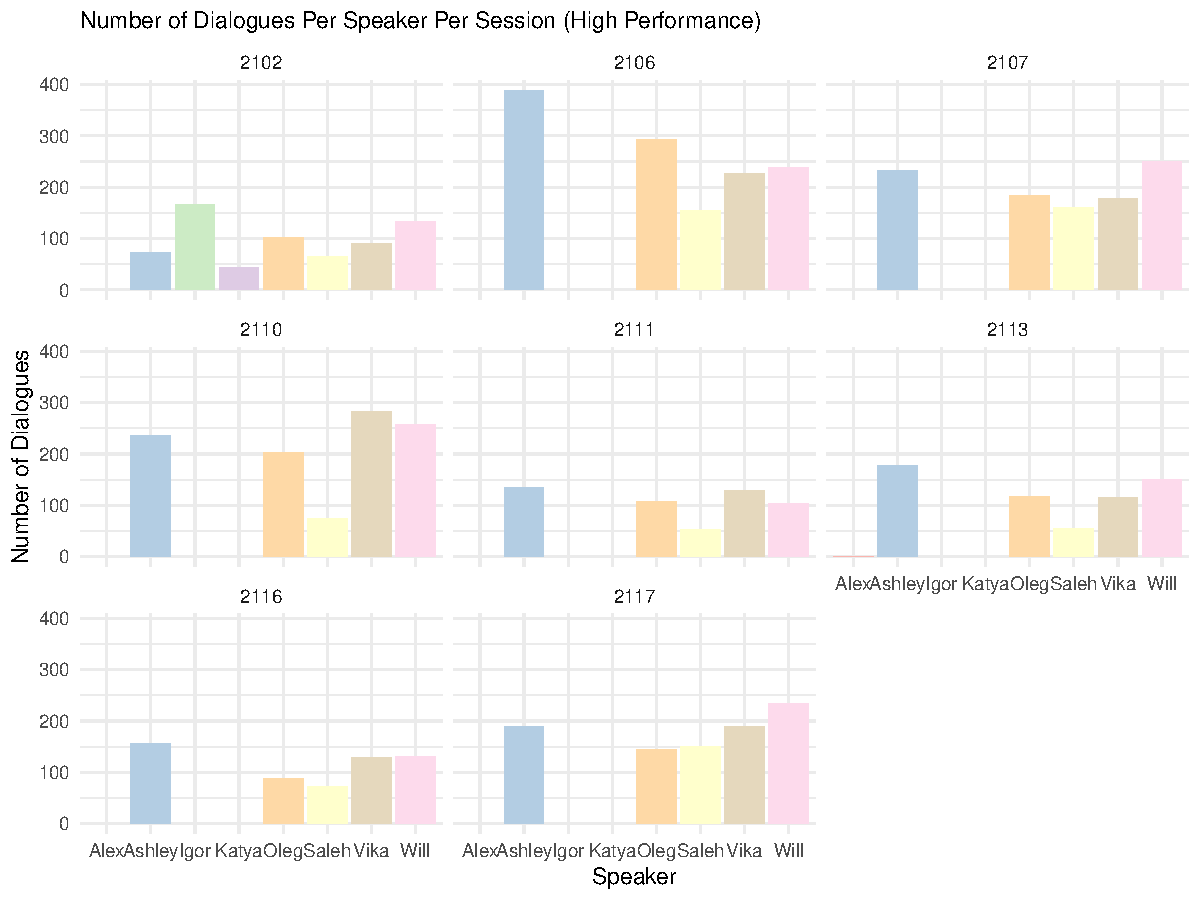
\includegraphics{low_surv_analysis_files/figure-latex/unnamed-chunk-4-1} \end{center}

\begin{Shaded}
\begin{Highlighting}[]
\NormalTok{total\_dialogues\_per\_speaker }\OtherTok{\textless{}{-}}\NormalTok{ low\_perf\_interactions }\SpecialCharTok{\%\textgreater{}\%}
  \FunctionTok{left\_join}\NormalTok{(actors\_attributes, }\AttributeTok{by =} \FunctionTok{c}\NormalTok{(}\StringTok{"sender\_id"} \OtherTok{=} \StringTok{"id"}\NormalTok{)) }\SpecialCharTok{\%\textgreater{}\%}
  \FunctionTok{group\_by}\NormalTok{(name) }\SpecialCharTok{\%\textgreater{}\%}
  \FunctionTok{summarise}\NormalTok{(}\AttributeTok{number\_of\_dialogues =} \FunctionTok{n}\NormalTok{(), }\AttributeTok{.groups =} \StringTok{\textquotesingle{}drop\textquotesingle{}}\NormalTok{) }\SpecialCharTok{\%\textgreater{}\%}
  \FunctionTok{arrange}\NormalTok{(}\FunctionTok{desc}\NormalTok{(number\_of\_dialogues)) }\SpecialCharTok{\%\textgreater{}\%}  \FunctionTok{as\_tibble}\NormalTok{() }
\NormalTok{total\_dialogues\_per\_speaker }\SpecialCharTok{\%\textgreater{}\%} \FunctionTok{print}\NormalTok{()}
\end{Highlighting}
\end{Shaded}

\begin{verbatim}
## # A tibble: 8 x 2
##   name   number_of_dialogues
##   <chr>                <int>
## 1 Ashley                1590
## 2 Will                  1500
## 3 Vika                  1341
## 4 Oleg                  1238
## 5 Saleh                  782
## 6 Igor                   167
## 7 Katya                   44
## 8 Alex                     1
\end{verbatim}

\begin{Shaded}
\begin{Highlighting}[]
\FunctionTok{ggplot}\NormalTok{(total\_dialogues\_per\_speaker, }\FunctionTok{aes}\NormalTok{(}\AttributeTok{x =}\NormalTok{ name, }\AttributeTok{y =}\NormalTok{ number\_of\_dialogues, }\AttributeTok{fill =}\NormalTok{ name)) }\SpecialCharTok{+} 
  \FunctionTok{geom\_bar}\NormalTok{(}\AttributeTok{stat =} \StringTok{"identity"}\NormalTok{) }\SpecialCharTok{+}
  \FunctionTok{scale\_fill\_brewer}\NormalTok{(}\AttributeTok{palette =} \StringTok{"Pastel1"}\NormalTok{) }\SpecialCharTok{+}  
  \FunctionTok{labs}\NormalTok{(}\AttributeTok{subtitle =} \StringTok{"Number of Dialogues Per Speaker Per Session (High Performance)"}\NormalTok{,}
       \AttributeTok{x =} \StringTok{"Speaker"}\NormalTok{,}
       \AttributeTok{y =} \StringTok{"Number of Dialogues"}\NormalTok{,}
       \AttributeTok{fill =} \StringTok{"Speaker"}\NormalTok{) }\SpecialCharTok{+}
  \FunctionTok{theme\_minimal}\NormalTok{() }\SpecialCharTok{+} 
  \FunctionTok{theme}\NormalTok{(}\AttributeTok{legend.position =} \StringTok{"none"}\NormalTok{) }
\end{Highlighting}
\end{Shaded}

\begin{center}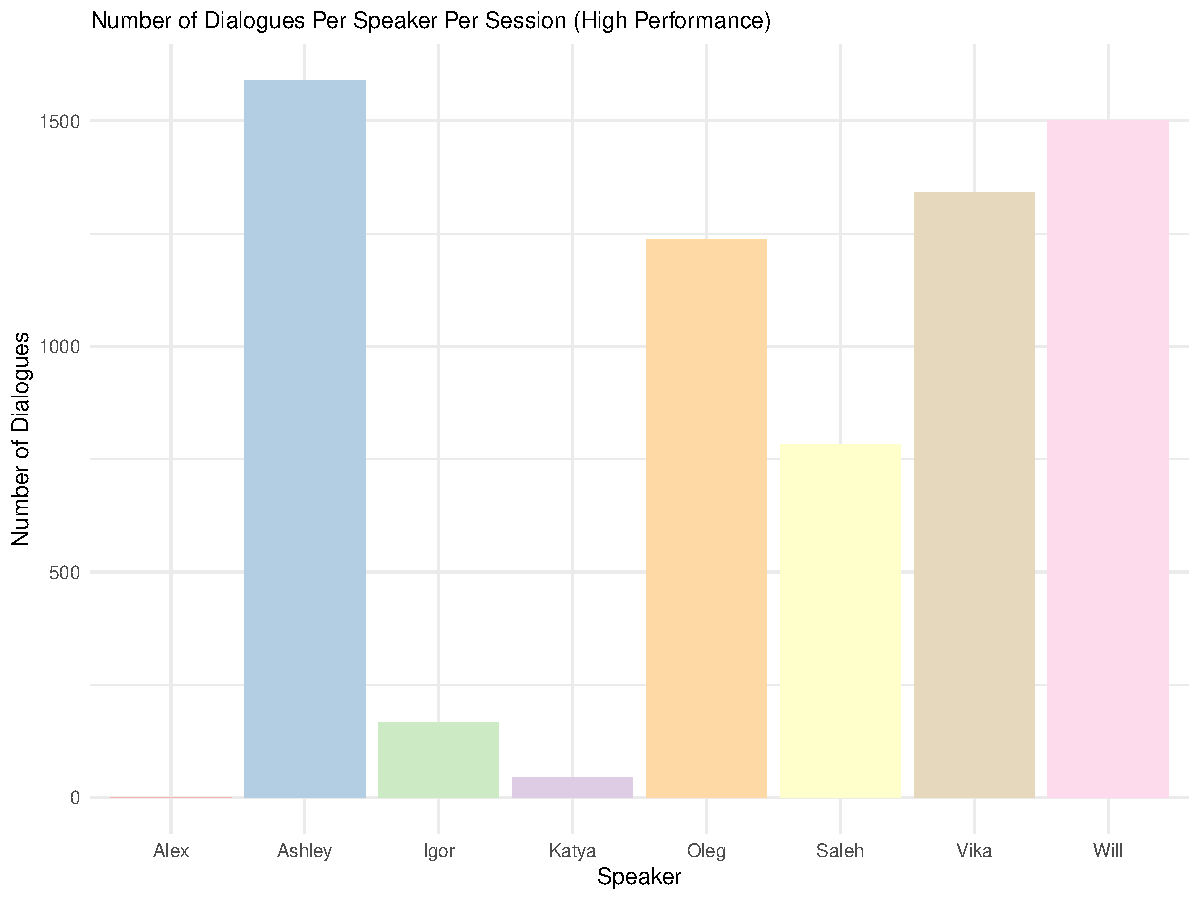
\includegraphics{low_surv_analysis_files/figure-latex/unnamed-chunk-6-1} \end{center}

\begin{Shaded}
\begin{Highlighting}[]
\NormalTok{dialog\_colors }\OtherTok{\textless{}{-}}\NormalTok{ RColorBrewer}\SpecialCharTok{::}\FunctionTok{brewer.pal}\NormalTok{(}\AttributeTok{n =} \FunctionTok{length}\NormalTok{(}\FunctionTok{unique}\NormalTok{(interactions}\SpecialCharTok{$}\NormalTok{dialog)), }\AttributeTok{name =} \StringTok{"Pastel2"}\NormalTok{)}
\NormalTok{dialog\_color\_map }\OtherTok{\textless{}{-}} \FunctionTok{setNames}\NormalTok{(dialog\_colors, }\FunctionTok{unique}\NormalTok{(interactions}\SpecialCharTok{$}\NormalTok{dialog))}

\NormalTok{low\_perf\_interactions }\SpecialCharTok{\%\textgreater{}\%} \FunctionTok{filter}\NormalTok{(receiver\_id }\SpecialCharTok{!=} \DecValTok{0}\NormalTok{)  }\SpecialCharTok{\%\textgreater{}\%} \FunctionTok{select}\NormalTok{(}\SpecialCharTok{{-}}\NormalTok{session) }\SpecialCharTok{\%\textgreater{}\%} \FunctionTok{mutate}\NormalTok{(}\AttributeTok{time =} \DecValTok{1}\SpecialCharTok{:}\FunctionTok{nrow}\NormalTok{(.))  }\SpecialCharTok{\%\textgreater{}\%} \FunctionTok{select}\NormalTok{(sender\_id, receiver\_id, time,dialog)  }\SpecialCharTok{\%\textgreater{}\%} \FunctionTok{mutate}\NormalTok{(}\AttributeTok{dialog =} \FunctionTok{as.factor}\NormalTok{(dialog), }\AttributeTok{sender\_id =} \FunctionTok{as.integer}\NormalTok{(sender\_id), }\AttributeTok{receiver\_id =} \FunctionTok{as.integer}\NormalTok{(receiver\_id)) }\OtherTok{{-}\textgreater{}}\NormalTok{ interactions}

\NormalTok{actors\_attributes }\SpecialCharTok{\%\textgreater{}\%} \FunctionTok{filter}\NormalTok{(id }\SpecialCharTok{\%in\%}\NormalTok{ interactions}\SpecialCharTok{$}\NormalTok{sender\_id) }\SpecialCharTok{\%\textgreater{}\%} \FunctionTok{filter}\NormalTok{(id }\SpecialCharTok{\%in\%}\NormalTok{ interactions}\SpecialCharTok{$}\NormalTok{receiver\_id) }\OtherTok{{-}\textgreater{}}\NormalTok{ actors\_attributes}
\FunctionTok{head}\NormalTok{(actors\_attributes)}
\end{Highlighting}
\end{Shaded}

\begin{verbatim}
##   id   name gendermale
## 1  1   Igor          1
## 2  2 Ashley          0
## 3  3   Will          1
## 4  4  Katya          0
## 5  5  Saleh          1
## 6  6   Oleg          1
\end{verbatim}

\begin{Shaded}
\begin{Highlighting}[]
\NormalTok{g\_subset }\OtherTok{\textless{}{-}} \FunctionTok{graph\_from\_data\_frame}\NormalTok{(interactions, }\AttributeTok{directed =} \ConstantTok{TRUE}\NormalTok{, }\AttributeTok{vertices =} \FunctionTok{data.frame}\NormalTok{(actors\_attributes))}


\FunctionTok{V}\NormalTok{(g\_subset)}\SpecialCharTok{$}\NormalTok{gender }\OtherTok{\textless{}{-}}\NormalTok{ actors\_attributes}\SpecialCharTok{$}\NormalTok{gender[}\FunctionTok{match}\NormalTok{(}\FunctionTok{V}\NormalTok{(g\_subset)}\SpecialCharTok{$}\NormalTok{name, actors\_attributes}\SpecialCharTok{$}\NormalTok{name)]}
\FunctionTok{V}\NormalTok{(g\_subset)}\SpecialCharTok{$}\NormalTok{name }\OtherTok{\textless{}{-}}\NormalTok{ actors\_attributes}\SpecialCharTok{$}\NormalTok{name[}\FunctionTok{match}\NormalTok{(}\FunctionTok{V}\NormalTok{(g\_subset)}\SpecialCharTok{$}\NormalTok{name, actors\_attributes}\SpecialCharTok{$}\NormalTok{name)]}
\FunctionTok{ggraph}\NormalTok{(g\_subset, }\AttributeTok{layout =} \StringTok{\textquotesingle{}fr\textquotesingle{}}\NormalTok{) }\SpecialCharTok{+}
  \FunctionTok{geom\_edge\_link}\NormalTok{(}\FunctionTok{aes}\NormalTok{(}\AttributeTok{color =}\NormalTok{ dialog), }\AttributeTok{alpha =} \FloatTok{0.7}\NormalTok{, }\AttributeTok{edge\_width =}\NormalTok{ .}\DecValTok{2}\NormalTok{, }\AttributeTok{lineend =} \StringTok{"butt"}\NormalTok{, }\AttributeTok{arrow =} \FunctionTok{arrow}\NormalTok{(}\AttributeTok{type =} \StringTok{\textquotesingle{}closed\textquotesingle{}}\NormalTok{, }\AttributeTok{length =} \FunctionTok{unit}\NormalTok{(}\DecValTok{4}\NormalTok{, }\StringTok{\textquotesingle{}mm\textquotesingle{}}\NormalTok{))) }\SpecialCharTok{+}
  \FunctionTok{scale\_edge\_color\_manual}\NormalTok{(}\AttributeTok{values =}\NormalTok{ dialog\_color\_map) }\SpecialCharTok{+}
  \FunctionTok{geom\_node\_point}\NormalTok{(}\FunctionTok{aes}\NormalTok{(}\AttributeTok{color =} \FunctionTok{factor}\NormalTok{(gender)), }\AttributeTok{size =} \DecValTok{4}\NormalTok{, }\AttributeTok{alpha =} \FloatTok{0.8}\NormalTok{) }\SpecialCharTok{+}
  \FunctionTok{geom\_node\_text}\NormalTok{(}\FunctionTok{aes}\NormalTok{(}\AttributeTok{label =}\NormalTok{ name), }\AttributeTok{repel =} \ConstantTok{TRUE}\NormalTok{,  }\AttributeTok{color =} \StringTok{"black"}\NormalTok{, }\AttributeTok{size =} \DecValTok{3}\NormalTok{, }\AttributeTok{vjust =} \DecValTok{1}\NormalTok{, }\AttributeTok{nudge\_x =} \SpecialCharTok{{-}}\NormalTok{.}\DecValTok{02}\NormalTok{) }\SpecialCharTok{+}
  \FunctionTok{scale\_color\_manual}\NormalTok{(}\AttributeTok{values =} \FunctionTok{c}\NormalTok{(}\StringTok{\textquotesingle{}0\textquotesingle{}} \OtherTok{=} \StringTok{\textquotesingle{}red\textquotesingle{}}\NormalTok{, }\StringTok{\textquotesingle{}1\textquotesingle{}} \OtherTok{=} \StringTok{\textquotesingle{}cyan\textquotesingle{}}\NormalTok{)) }\SpecialCharTok{+}
  \FunctionTok{theme\_void}\NormalTok{() }\SpecialCharTok{+}
  \FunctionTok{labs}\NormalTok{(}\AttributeTok{subtitle =} \StringTok{"High Performing Session 2104"}\NormalTok{, }\AttributeTok{color =} \StringTok{"Gender"}\NormalTok{, }\AttributeTok{edge\_color =} \StringTok{"Dialog"}\NormalTok{) }\SpecialCharTok{+}
  \FunctionTok{theme}\NormalTok{(}\AttributeTok{legend.position =} \StringTok{"right"}\NormalTok{, }\AttributeTok{legend.title =} \FunctionTok{element\_text}\NormalTok{(}\AttributeTok{size =} \DecValTok{8}\NormalTok{))}
\end{Highlighting}
\end{Shaded}

\begin{center}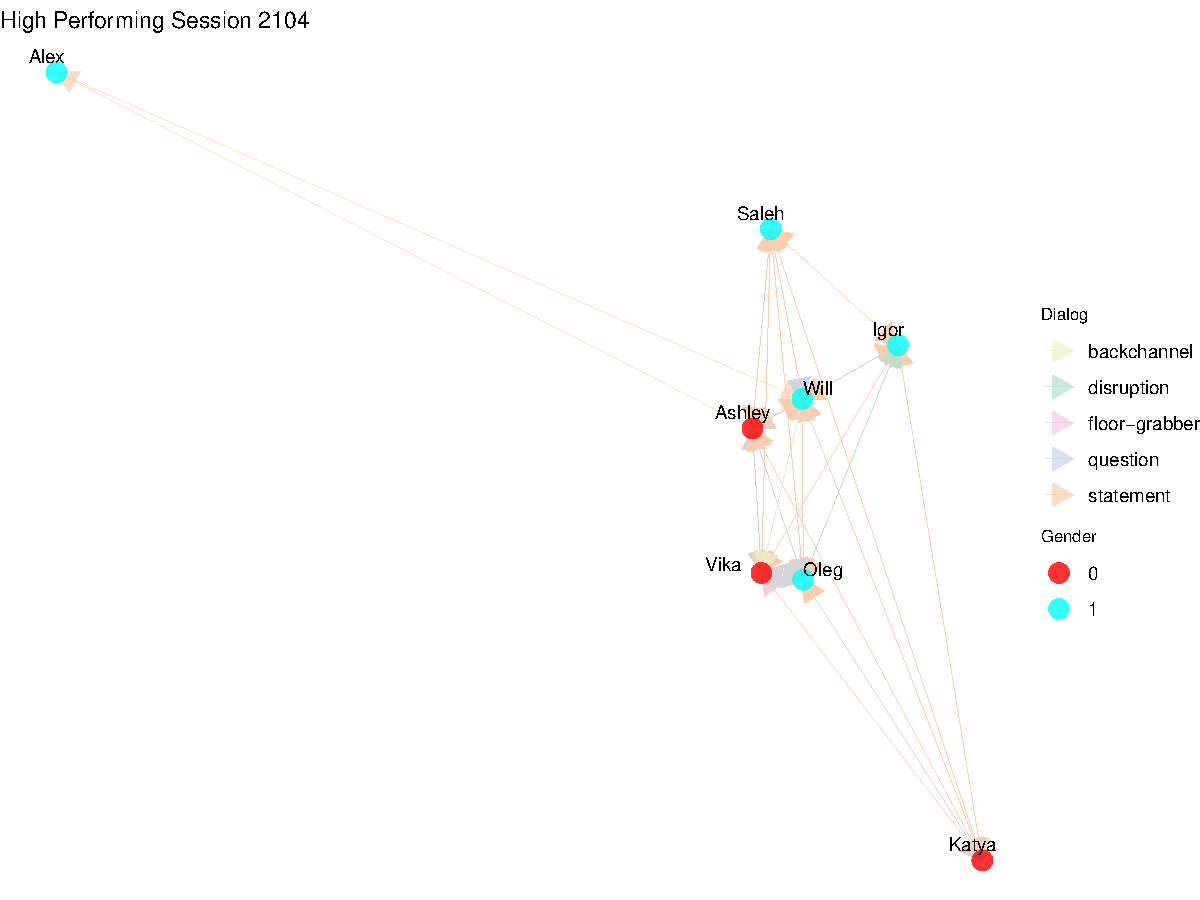
\includegraphics{low_surv_analysis_files/figure-latex/unnamed-chunk-7-1} \end{center}

\begin{Shaded}
\begin{Highlighting}[]
\CommentTok{\# remove alex from sender\_id}
\NormalTok{actors\_attributes }\SpecialCharTok{\%\textgreater{}\%} \FunctionTok{filter}\NormalTok{(name }\SpecialCharTok{!=} \StringTok{"Alex"}\NormalTok{) }\OtherTok{{-}\textgreater{}}\NormalTok{ actors\_attributes}

\NormalTok{low\_perf\_interactions }\SpecialCharTok{\%\textgreater{}\%} \FunctionTok{filter}\NormalTok{(receiver\_id }\SpecialCharTok{!=} \DecValTok{0}\NormalTok{) }\SpecialCharTok{\%\textgreater{}\%} \FunctionTok{select}\NormalTok{(}\SpecialCharTok{{-}}\NormalTok{session) }\SpecialCharTok{\%\textgreater{}\%} \FunctionTok{mutate}\NormalTok{(}\AttributeTok{time =} \DecValTok{1}\SpecialCharTok{:}\FunctionTok{nrow}\NormalTok{(.))  }\SpecialCharTok{\%\textgreater{}\%} \FunctionTok{select}\NormalTok{(sender\_id, receiver\_id, time,dialog)  }\SpecialCharTok{\%\textgreater{}\%} \FunctionTok{mutate}\NormalTok{(}\AttributeTok{dialog =} \FunctionTok{as.factor}\NormalTok{(dialog), }\AttributeTok{sender\_id =} \FunctionTok{as.integer}\NormalTok{(sender\_id), }\AttributeTok{receiver\_id =} \FunctionTok{as.integer}\NormalTok{(receiver\_id)) }\OtherTok{{-}\textgreater{}}\NormalTok{ interactions}

\NormalTok{actors\_attributes }\SpecialCharTok{\%\textgreater{}\%} \FunctionTok{filter}\NormalTok{(id }\SpecialCharTok{\%in\%}\NormalTok{ interactions}\SpecialCharTok{$}\NormalTok{sender\_id) }\SpecialCharTok{\%\textgreater{}\%} \FunctionTok{filter}\NormalTok{(id }\SpecialCharTok{\%in\%}\NormalTok{ interactions}\SpecialCharTok{$}\NormalTok{receiver\_id) }\OtherTok{{-}\textgreater{}}\NormalTok{ actors\_attributes}
\FunctionTok{head}\NormalTok{(actors\_attributes)}
\end{Highlighting}
\end{Shaded}

\begin{verbatim}
##   id   name gendermale
## 1  1   Igor          1
## 2  2 Ashley          0
## 3  3   Will          1
## 4  4  Katya          0
## 5  5  Saleh          1
## 6  6   Oleg          1
\end{verbatim}

\begin{Shaded}
\begin{Highlighting}[]
\NormalTok{low\_perf\_interactions }\SpecialCharTok{\%\textgreater{}\%} \FunctionTok{filter}\NormalTok{(receiver\_id }\SpecialCharTok{!=} \DecValTok{0}\NormalTok{) }\SpecialCharTok{\%\textgreater{}\%} \FunctionTok{select}\NormalTok{(}\SpecialCharTok{{-}}\NormalTok{session) }\SpecialCharTok{\%\textgreater{}\%} \FunctionTok{mutate}\NormalTok{(}\AttributeTok{time =} \DecValTok{1}\SpecialCharTok{:}\FunctionTok{nrow}\NormalTok{(.))  }\SpecialCharTok{\%\textgreater{}\%} \FunctionTok{select}\NormalTok{(sender\_id, receiver\_id, time,dialog)  }\SpecialCharTok{\%\textgreater{}\%} \FunctionTok{mutate}\NormalTok{(}\AttributeTok{dialog =} \FunctionTok{as.factor}\NormalTok{(dialog), }\AttributeTok{sender\_id =} \FunctionTok{as.integer}\NormalTok{(sender\_id), }\AttributeTok{receiver\_id =} \FunctionTok{as.integer}\NormalTok{(receiver\_id)) }\SpecialCharTok{\%\textgreater{}\%} \FunctionTok{filter}\NormalTok{(sender\_id }\SpecialCharTok{\%in\%}\NormalTok{ actors\_attributes}\SpecialCharTok{$}\NormalTok{id) }\SpecialCharTok{\%\textgreater{}\%} \FunctionTok{filter}\NormalTok{(receiver\_id }\SpecialCharTok{\%in\%}\NormalTok{ actors\_attributes}\SpecialCharTok{$}\NormalTok{id) }\OtherTok{{-}\textgreater{}}\NormalTok{ interactions}

\FunctionTok{dim}\NormalTok{(interactions)}
\end{Highlighting}
\end{Shaded}

\begin{verbatim}
## [1] 6655    4
\end{verbatim}

\begin{Shaded}
\begin{Highlighting}[]
\FunctionTok{head}\NormalTok{(interactions)}
\end{Highlighting}
\end{Shaded}

\begin{verbatim}
## # A tibble: 6 x 4
##   sender_id receiver_id  time dialog    
##       <int>       <int> <int> <fct>     
## 1         1           2     1 disruption
## 2         2           3     2 statement 
## 3         3           1     3 question  
## 4         1           2     4 statement 
## 5         2           1     5 statement 
## 6         1           3     6 statement
\end{verbatim}

\begin{Shaded}
\begin{Highlighting}[]
\NormalTok{actors\_attributes }\SpecialCharTok{\%\textgreater{}\%} \FunctionTok{filter}\NormalTok{(id }\SpecialCharTok{\%in\%}\NormalTok{ interactions}\SpecialCharTok{$}\NormalTok{sender\_id) }\SpecialCharTok{\%\textgreater{}\%} \FunctionTok{filter}\NormalTok{(id }\SpecialCharTok{\%in\%}\NormalTok{ interactions}\SpecialCharTok{$}\NormalTok{receiver\_id) }\OtherTok{{-}\textgreater{}}\NormalTok{ actors\_attributes}

\NormalTok{g\_subset }\OtherTok{\textless{}{-}} \FunctionTok{graph\_from\_data\_frame}\NormalTok{(interactions, }\AttributeTok{directed =} \ConstantTok{TRUE}\NormalTok{, }\AttributeTok{vertices =} \FunctionTok{data.frame}\NormalTok{(actors\_attributes))}


\FunctionTok{V}\NormalTok{(g\_subset)}\SpecialCharTok{$}\NormalTok{gender }\OtherTok{\textless{}{-}}\NormalTok{ actors\_attributes}\SpecialCharTok{$}\NormalTok{gender[}\FunctionTok{match}\NormalTok{(}\FunctionTok{V}\NormalTok{(g\_subset)}\SpecialCharTok{$}\NormalTok{name, actors\_attributes}\SpecialCharTok{$}\NormalTok{name)]}
\FunctionTok{V}\NormalTok{(g\_subset)}\SpecialCharTok{$}\NormalTok{name }\OtherTok{\textless{}{-}}\NormalTok{ actors\_attributes}\SpecialCharTok{$}\NormalTok{name[}\FunctionTok{match}\NormalTok{(}\FunctionTok{V}\NormalTok{(g\_subset)}\SpecialCharTok{$}\NormalTok{name, actors\_attributes}\SpecialCharTok{$}\NormalTok{name)]}
\end{Highlighting}
\end{Shaded}

\begin{Shaded}
\begin{Highlighting}[]
\NormalTok{interactions}\SpecialCharTok{$}\NormalTok{time}\OtherTok{\textless{}{-}}\FunctionTok{as.numeric}\NormalTok{(interactions}\SpecialCharTok{$}\NormalTok{time) }


\NormalTok{REM.data }\OtherTok{\textless{}{-}} \FunctionTok{createRemDataset}\NormalTok{(}
  \AttributeTok{data =}\NormalTok{ interactions, }
  \AttributeTok{sender =}\NormalTok{ interactions}\SpecialCharTok{$}\NormalTok{sender\_id,}
  \AttributeTok{target =}\NormalTok{ interactions}\SpecialCharTok{$}\NormalTok{receiver\_id,}
  \AttributeTok{eventSequence =}\NormalTok{ interactions}\SpecialCharTok{$}\NormalTok{time,}
  \AttributeTok{eventAttribute =}\NormalTok{ interactions}\SpecialCharTok{$}\NormalTok{dialog,}
  \AttributeTok{atEventTimesOnly =} \ConstantTok{TRUE}\NormalTok{, }
  \AttributeTok{untilEventOccurrs =} \ConstantTok{TRUE}\NormalTok{,}
  \AttributeTok{includeAllPossibleEvents =} \ConstantTok{FALSE}\NormalTok{, }
  \AttributeTok{returnInputData =} \ConstantTok{FALSE}
\NormalTok{)}

\CommentTok{\#save as RDS}
\CommentTok{\#saveRDS(REM.data, "data/RemDatasetLow.RDS")}
\end{Highlighting}
\end{Shaded}

\begin{Shaded}
\begin{Highlighting}[]
\FunctionTok{readRDS}\NormalTok{(}\StringTok{"data/REM\_data.RDS"}\NormalTok{) }\OtherTok{{-}\textgreater{}}\NormalTok{ REM.data}
\end{Highlighting}
\end{Shaded}

\begin{Shaded}
\begin{Highlighting}[]
\FunctionTok{dim}\NormalTok{(REM.data)}
\end{Highlighting}
\end{Shaded}

\begin{verbatim}
## [1] 90290    12
\end{verbatim}

\begin{Shaded}
\begin{Highlighting}[]
\FunctionTok{str}\NormalTok{(REM.data)}
\end{Highlighting}
\end{Shaded}

\begin{verbatim}
## 'data.frame':    90290 obs. of  12 variables:
##  $ target          : chr  "2" "2" "2" "2" ...
##  $ sender          : chr  "2" "3" "3" "6" ...
##  $ eventID         : chr  "eventID1" "eventID96" "eventID96" "eventID969" ...
##  $ eventTime       : num  1 38 39 959 960 961 962 179 180 181 ...
##  $ eventDummy      : num  1 0 0 0 0 0 0 0 0 0 ...
##  $ eventAtRiskFrom : num  1 1 1 949 949 949 949 1 1 1 ...
##  $ eventAtRiskUntil: num  1 96 96 969 969 969 969 199 199 199 ...
##  $ eventAttribute  : chr  "disruption" "statement" "statement" "statement" ...
##  $ name.x          : chr  "Ashley" "Will" "Will" "Oleg" ...
##  $ gendermale.x    : num  0 1 1 1 1 1 1 0 0 0 ...
##  $ name.y          : chr  "Ashley" "Ashley" "Ashley" "Ashley" ...
##  $ gendermale.y    : num  0 0 0 0 0 0 0 0 0 0 ...
\end{verbatim}

\begin{Shaded}
\begin{Highlighting}[]
\NormalTok{surv\_object }\OtherTok{\textless{}{-}} \FunctionTok{Surv}\NormalTok{(}\AttributeTok{time =}\NormalTok{ REM.data}\SpecialCharTok{$}\NormalTok{eventTime, }\AttributeTok{event =}\NormalTok{ REM.data}\SpecialCharTok{$}\NormalTok{eventDummy)}
\end{Highlighting}
\end{Shaded}

\begin{Shaded}
\begin{Highlighting}[]
\NormalTok{base\_model }\OtherTok{\textless{}{-}} \FunctionTok{coxph}\NormalTok{(surv\_object }\SpecialCharTok{\textasciitilde{}} \DecValTok{1}\NormalTok{, }\AttributeTok{data =}\NormalTok{ REM.data)}
\FunctionTok{summary}\NormalTok{(base\_model)}
\end{Highlighting}
\end{Shaded}

\begin{verbatim}
## Call:  coxph(formula = surv_object ~ 1, data = REM.data)
## 
## Null model
##   log likelihood= -9798.436 
##   n= 90290
\end{verbatim}

\begin{Shaded}
\begin{Highlighting}[]
\NormalTok{sender\_model }\OtherTok{\textless{}{-}} \FunctionTok{coxph}\NormalTok{(surv\_object }\SpecialCharTok{\textasciitilde{}}\NormalTok{ sender }\SpecialCharTok{+} \DecValTok{1}\NormalTok{, }\AttributeTok{data =}\NormalTok{ REM.data)}


\FunctionTok{summary}\NormalTok{(sender\_model)}
\end{Highlighting}
\end{Shaded}

\begin{verbatim}
## Call:
## coxph(formula = surv_object ~ sender + 1, data = REM.data)
## 
##   n= 90290, number of events= 986 
## 
##             coef exp(coef) se(coef)      z Pr(>|z|)    
## sender3 -0.32765   0.72062  0.09916 -3.304 0.000952 ***
## sender4 -0.23043   0.79419  0.10508 -2.193 0.028315 *  
## sender5 -0.66512   0.51421  0.12440 -5.347 8.96e-08 ***
## sender6 -0.33555   0.71495  0.09907 -3.387 0.000706 ***
## sender7 -0.32023   0.72598  0.10409 -3.076 0.002095 ** 
## ---
## Signif. codes:  0 '***' 0.001 '**' 0.01 '*' 0.05 '.' 0.1 ' ' 1
## 
##         exp(coef) exp(-coef) lower .95 upper .95
## sender3    0.7206      1.388    0.5933    0.8752
## sender4    0.7942      1.259    0.6464    0.9758
## sender5    0.5142      1.945    0.4029    0.6562
## sender6    0.7149      1.399    0.5888    0.8682
## sender7    0.7260      1.377    0.5920    0.8903
## 
## Concordance= 0.559  (se = 0.011 )
## Likelihood ratio test= 33.56  on 5 df,   p=3e-06
## Wald test            = 33.07  on 5 df,   p=4e-06
## Score (logrank) test = 33.65  on 5 df,   p=3e-06
\end{verbatim}

\begin{Shaded}
\begin{Highlighting}[]
\NormalTok{rec\_model }\OtherTok{\textless{}{-}} \FunctionTok{coxph}\NormalTok{(surv\_object }\SpecialCharTok{\textasciitilde{}}\NormalTok{ target }\SpecialCharTok{+} \DecValTok{1}\NormalTok{, }\AttributeTok{data =}\NormalTok{ REM.data)}


\FunctionTok{summary}\NormalTok{(rec\_model)}
\end{Highlighting}
\end{Shaded}

\begin{verbatim}
## Call:
## coxph(formula = surv_object ~ target + 1, data = REM.data)
## 
##   n= 90290, number of events= 986 
## 
##             coef exp(coef) se(coef)      z Pr(>|z|)    
## target3 -0.31147   0.73237  0.09916 -3.141  0.00168 ** 
## target4 -0.05321   0.94818  0.10539 -0.505  0.61366    
## target5 -0.58970   0.55449  0.12453 -4.735 2.19e-06 ***
## target6 -0.41861   0.65796  0.09931 -4.215 2.49e-05 ***
## target7 -0.07277   0.92981  0.10402 -0.700  0.48419    
## ---
## Signif. codes:  0 '***' 0.001 '**' 0.01 '*' 0.05 '.' 0.1 ' ' 1
## 
##         exp(coef) exp(-coef) lower .95 upper .95
## target3    0.7324      1.365    0.6030    0.8895
## target4    0.9482      1.055    0.7712    1.1657
## target5    0.5545      1.803    0.4344    0.7078
## target6    0.6580      1.520    0.5416    0.7993
## target7    0.9298      1.075    0.7583    1.1401
## 
## Concordance= 0.566  (se = 0.011 )
## Likelihood ratio test= 40.48  on 5 df,   p=1e-07
## Wald test            = 39.3  on 5 df,   p=2e-07
## Score (logrank) test = 39.94  on 5 df,   p=2e-07
\end{verbatim}

\begin{Shaded}
\begin{Highlighting}[]
\NormalTok{snd\_rec\_model }\OtherTok{\textless{}{-}} \FunctionTok{coxph}\NormalTok{(surv\_object }\SpecialCharTok{\textasciitilde{}}\NormalTok{ sender }\SpecialCharTok{+}\NormalTok{ target }\SpecialCharTok{+} \DecValTok{1}\NormalTok{, }\AttributeTok{data =}\NormalTok{ REM.data)}
\FunctionTok{summary}\NormalTok{(snd\_rec\_model)}
\end{Highlighting}
\end{Shaded}

\begin{verbatim}
## Call:
## coxph(formula = surv_object ~ sender + target + 1, data = REM.data)
## 
##   n= 90290, number of events= 986 
## 
##            coef exp(coef) se(coef)      z Pr(>|z|)    
## sender3 -0.4268    0.6526   0.1033 -4.131 3.62e-05 ***
## sender4 -0.2163    0.8055   0.1072 -2.018   0.0436 *  
## sender5 -0.8191    0.4408   0.1267 -6.463 1.03e-10 ***
## sender6 -0.4809    0.6182   0.1024 -4.697 2.63e-06 ***
## sender7 -0.4295    0.6509   0.1070 -4.015 5.94e-05 ***
## target3 -0.4370    0.6460   0.1033 -4.230 2.34e-05 ***
## target4 -0.1341    0.8745   0.1077 -1.245   0.2131    
## target5 -0.7362    0.4789   0.1270 -5.798 6.72e-09 ***
## target6 -0.5767    0.5617   0.1027 -5.618 1.94e-08 ***
## target7 -0.1409    0.8686   0.1053 -1.339   0.1807    
## ---
## Signif. codes:  0 '***' 0.001 '**' 0.01 '*' 0.05 '.' 0.1 ' ' 1
## 
##         exp(coef) exp(-coef) lower .95 upper .95
## sender3    0.6526      1.532    0.5329    0.7991
## sender4    0.8055      1.241    0.6529    0.9938
## sender5    0.4408      2.268    0.3439    0.5651
## sender6    0.6182      1.618    0.5058    0.7556
## sender7    0.6509      1.536    0.5278    0.8026
## target3    0.6460      1.548    0.5275    0.7910
## target4    0.8745      1.143    0.7081    1.0800
## target5    0.4789      2.088    0.3734    0.6143
## target6    0.5617      1.780    0.4593    0.6869
## target7    0.8686      1.151    0.7067    1.0676
## 
## Concordance= 0.606  (se = 0.011 )
## Likelihood ratio test= 93.47  on 10 df,   p=1e-15
## Wald test            = 90.93  on 10 df,   p=4e-15
## Score (logrank) test = 92.43  on 10 df,   p=2e-15
\end{verbatim}

\begin{Shaded}
\begin{Highlighting}[]
\NormalTok{event\_model }\OtherTok{\textless{}{-}} \FunctionTok{coxph}\NormalTok{(surv\_object }\SpecialCharTok{\textasciitilde{}}\NormalTok{ eventAttribute }\SpecialCharTok{+} \DecValTok{1}\NormalTok{, }\AttributeTok{data =}\NormalTok{ REM.data)}
\FunctionTok{summary}\NormalTok{(event\_model)}
\end{Highlighting}
\end{Shaded}

\begin{verbatim}
## Call:
## coxph(formula = surv_object ~ eventAttribute + 1, data = REM.data)
## 
##   n= 90290, number of events= 986 
## 
##                               coef exp(coef) se(coef)     z Pr(>|z|)    
## eventAttributedisruption    0.1617    1.1755   0.2717 0.595    0.552    
## eventAttributefloor-grabber 0.3357    1.3989   0.2273 1.477    0.140    
## eventAttributequestion      0.9340    2.5447   0.1853 5.041 4.63e-07 ***
## eventAttributestatement     1.4839    4.4099   0.1789 8.294  < 2e-16 ***
## ---
## Signif. codes:  0 '***' 0.001 '**' 0.01 '*' 0.05 '.' 0.1 ' ' 1
## 
##                             exp(coef) exp(-coef) lower .95 upper .95
## eventAttributedisruption        1.176     0.8507    0.6901     2.002
## eventAttributefloor-grabber     1.399     0.7148    0.8961     2.184
## eventAttributequestion          2.545     0.3930    1.7698     3.659
## eventAttributestatement         4.410     0.2268    3.1056     6.262
## 
## Concordance= 0.641  (se = 0.009 )
## Likelihood ratio test= 207  on 4 df,   p=<2e-16
## Wald test            = 172.3  on 4 df,   p=<2e-16
## Score (logrank) test = 190.6  on 4 df,   p=<2e-16
\end{verbatim}

\begin{Shaded}
\begin{Highlighting}[]
\NormalTok{model4 }\OtherTok{\textless{}{-}} \FunctionTok{coxph}\NormalTok{(surv\_object }\SpecialCharTok{\textasciitilde{}}\NormalTok{ sender }\SpecialCharTok{+}\NormalTok{ eventAttribute, }\AttributeTok{data =}\NormalTok{ REM.data)}
\FunctionTok{summary}\NormalTok{(model4)}
\end{Highlighting}
\end{Shaded}

\begin{verbatim}
## Call:
## coxph(formula = surv_object ~ sender + eventAttribute, data = REM.data)
## 
##   n= 90290, number of events= 986 
## 
##                                 coef exp(coef) se(coef)      z Pr(>|z|)    
## sender3                     -0.32011   0.72607  0.09953 -3.216 0.001299 ** 
## sender4                     -0.36260   0.69586  0.10563 -3.433 0.000598 ***
## sender5                     -0.76721   0.46431  0.12467 -6.154 7.55e-10 ***
## sender6                     -0.49032   0.61243  0.09967 -4.919 8.68e-07 ***
## sender7                     -0.32726   0.72089  0.10440 -3.135 0.001720 ** 
## eventAttributedisruption     0.23939   1.27048  0.27340  0.876 0.381237    
## eventAttributefloor-grabber  0.38767   1.47355  0.22795  1.701 0.088995 .  
## eventAttributequestion       1.04592   2.84602  0.18777  5.570 2.55e-08 ***
## eventAttributestatement      1.58097   4.85967  0.18048  8.760  < 2e-16 ***
## ---
## Signif. codes:  0 '***' 0.001 '**' 0.01 '*' 0.05 '.' 0.1 ' ' 1
## 
##                             exp(coef) exp(-coef) lower .95 upper .95
## sender3                        0.7261     1.3773    0.5974    0.8825
## sender4                        0.6959     1.4371    0.5657    0.8559
## sender5                        0.4643     2.1538    0.3637    0.5928
## sender6                        0.6124     1.6328    0.5038    0.7446
## sender7                        0.7209     1.3872    0.5875    0.8846
## eventAttributedisruption       1.2705     0.7871    0.7434    2.1711
## eventAttributefloor-grabber    1.4735     0.6786    0.9426    2.3035
## eventAttributequestion         2.8460     0.3514    1.9697    4.1122
## eventAttributestatement        4.8597     0.2058    3.4118    6.9220
## 
## Concordance= 0.665  (se = 0.01 )
## Likelihood ratio test= 254.2  on 9 df,   p=<2e-16
## Wald test            = 219.7  on 9 df,   p=<2e-16
## Score (logrank) test = 238.7  on 9 df,   p=<2e-16
\end{verbatim}

\begin{Shaded}
\begin{Highlighting}[]
\NormalTok{model5 }\OtherTok{\textless{}{-}} \FunctionTok{coxph}\NormalTok{(surv\_object }\SpecialCharTok{\textasciitilde{}}\NormalTok{ sender }\SpecialCharTok{*}\NormalTok{ eventAttribute, }\AttributeTok{data =}\NormalTok{ REM.data)}
\FunctionTok{summary}\NormalTok{(model5)}
\end{Highlighting}
\end{Shaded}

\begin{verbatim}
## Call:
## coxph(formula = surv_object ~ sender * eventAttribute, data = REM.data)
## 
##   n= 90290, number of events= 986 
## 
##                                         coef exp(coef) se(coef)      z Pr(>|z|)
## sender3                             -0.33080   0.71835  0.50398 -0.656 0.511585
## sender4                              0.87067   2.38851  0.62777  1.387 0.165462
## sender5                              1.46375   4.32215  0.58731  2.492 0.012692
## sender6                              0.79299   2.20999  1.06982  0.741 0.458551
## sender7                              0.23690   1.26731  0.53462  0.443 0.657682
## eventAttributedisruption             0.95970   2.61091  0.47619  2.015 0.043865
## eventAttributefloor-grabber          1.00197   2.72363  0.44237  2.265 0.023513
## eventAttributequestion               1.43755   4.21037  0.40317  3.566 0.000363
## eventAttributestatement              1.95909   7.09285  0.38693  5.063 4.13e-07
## sender3:eventAttributedisruption    -0.06494   0.93712  0.81898 -0.079 0.936798
## sender4:eventAttributedisruption    -1.88494   0.15184  0.98907 -1.906 0.056680
## sender5:eventAttributedisruption    -3.83539   0.02159  1.19637 -3.206 0.001347
## sender6:eventAttributedisruption    -1.29988   0.27257  1.24935 -1.040 0.298136
## sender7:eventAttributedisruption    -1.33482   0.26321  0.93241 -1.432 0.152266
## sender3:eventAttributefloor-grabber -0.76328   0.46614  0.68799 -1.109 0.267247
## sender4:eventAttributefloor-grabber -1.35756   0.25729  0.83456 -1.627 0.103807
## sender5:eventAttributefloor-grabber -2.16281   0.11500  0.77238 -2.800 0.005107
## sender6:eventAttributefloor-grabber -1.22900   0.29259  1.15728 -1.062 0.288248
## sender7:eventAttributefloor-grabber -1.07158   0.34247  0.71085 -1.507 0.131691
## sender3:eventAttributequestion       0.30547   1.35727  0.54708  0.558 0.576595
## sender4:eventAttributequestion      -1.15034   0.31653  0.65948 -1.744 0.081104
## sender5:eventAttributequestion      -1.92038   0.14655  0.63087 -3.044 0.002334
## sender6:eventAttributequestion      -1.31403   0.26874  1.08797 -1.208 0.227133
## sender7:eventAttributequestion      -1.02853   0.35753  0.58170 -1.768 0.077039
## sender3:eventAttributestatement      0.02038   1.02059  0.51866  0.039 0.968650
## sender4:eventAttributestatement     -1.27119   0.28050  0.64208 -1.980 0.047726
## sender5:eventAttributestatement     -2.40823   0.08997  0.61037 -3.946 7.96e-05
## sender6:eventAttributestatement     -1.27692   0.27889  1.07713 -1.185 0.235824
## sender7:eventAttributestatement     -0.32597   0.72183  0.54960 -0.593 0.553109
##                                        
## sender3                                
## sender4                                
## sender5                             *  
## sender6                                
## sender7                                
## eventAttributedisruption            *  
## eventAttributefloor-grabber         *  
## eventAttributequestion              ***
## eventAttributestatement             ***
## sender3:eventAttributedisruption       
## sender4:eventAttributedisruption    .  
## sender5:eventAttributedisruption    ** 
## sender6:eventAttributedisruption       
## sender7:eventAttributedisruption       
## sender3:eventAttributefloor-grabber    
## sender4:eventAttributefloor-grabber    
## sender5:eventAttributefloor-grabber ** 
## sender6:eventAttributefloor-grabber    
## sender7:eventAttributefloor-grabber    
## sender3:eventAttributequestion         
## sender4:eventAttributequestion      .  
## sender5:eventAttributequestion      ** 
## sender6:eventAttributequestion         
## sender7:eventAttributequestion      .  
## sender3:eventAttributestatement        
## sender4:eventAttributestatement     *  
## sender5:eventAttributestatement     ***
## sender6:eventAttributestatement        
## sender7:eventAttributestatement        
## ---
## Signif. codes:  0 '***' 0.001 '**' 0.01 '*' 0.05 '.' 0.1 ' ' 1
## 
##                                     exp(coef) exp(-coef) lower .95 upper .95
## sender3                               0.71835     1.3921   0.26751    1.9290
## sender4                               2.38851     0.4187   0.69787    8.1749
## sender5                               4.32215     0.2314   1.36703   13.6654
## sender6                               2.20999     0.4525   0.27149   17.9896
## sender7                               1.26731     0.7891   0.44444    3.6137
## eventAttributedisruption              2.61091     0.3830   1.02674    6.6393
## eventAttributefloor-grabber           2.72363     0.3672   1.14446    6.4818
## eventAttributequestion                4.21037     0.2375   1.91047    9.2790
## eventAttributestatement               7.09285     0.1410   3.32247   15.1419
## sender3:eventAttributedisruption      0.93712     1.0671   0.18822    4.6657
## sender4:eventAttributedisruption      0.15184     6.5860   0.02185    1.0551
## sender5:eventAttributedisruption      0.02159    46.3116   0.00207    0.2253
## sender6:eventAttributedisruption      0.27257     3.6688   0.02355    3.1544
## sender7:eventAttributedisruption      0.26321     3.7993   0.04233    1.6367
## sender3:eventAttributefloor-grabber   0.46614     2.1453   0.12103    1.7953
## sender4:eventAttributefloor-grabber   0.25729     3.8867   0.05012    1.3207
## sender5:eventAttributefloor-grabber   0.11500     8.6955   0.02531    0.5226
## sender6:eventAttributefloor-grabber   0.29259     3.4178   0.03028    2.8270
## sender7:eventAttributefloor-grabber   0.34247     2.9200   0.08502    1.3794
## sender3:eventAttributequestion        1.35727     0.7368   0.46450    3.9659
## sender4:eventAttributequestion        0.31653     3.1593   0.08691    1.1528
## sender5:eventAttributequestion        0.14655     6.8236   0.04256    0.5046
## sender6:eventAttributequestion        0.26874     3.7211   0.03186    2.2668
## sender7:eventAttributequestion        0.35753     2.7969   0.11433    1.1181
## sender3:eventAttributestatement       1.02059     0.9798   0.36929    2.8206
## sender4:eventAttributestatement       0.28050     3.5651   0.07969    0.9873
## sender5:eventAttributestatement       0.08997    11.1143   0.02720    0.2976
## sender6:eventAttributestatement       0.27889     3.5856   0.03377    2.3030
## sender7:eventAttributestatement       0.72183     1.3854   0.24582    2.1196
## 
## Concordance= 0.675  (se = 0.01 )
## Likelihood ratio test= 300  on 29 df,   p=<2e-16
## Wald test            = 238.4  on 29 df,   p=<2e-16
## Score (logrank) test = 282.6  on 29 df,   p=<2e-16
\end{verbatim}

\begin{Shaded}
\begin{Highlighting}[]
\NormalTok{model6 }\OtherTok{\textless{}{-}} \FunctionTok{coxph}\NormalTok{(surv\_object }\SpecialCharTok{\textasciitilde{}}\NormalTok{ sender }\SpecialCharTok{+}\NormalTok{ target }\SpecialCharTok{+}\NormalTok{ eventAttribute, }\AttributeTok{data =}\NormalTok{ REM.data)}
\FunctionTok{summary}\NormalTok{(model6)}
\end{Highlighting}
\end{Shaded}

\begin{verbatim}
## Call:
## coxph(formula = surv_object ~ sender + target + eventAttribute, 
##     data = REM.data)
## 
##   n= 90290, number of events= 986 
## 
##                                coef exp(coef) se(coef)      z Pr(>|z|)    
## sender3                     -0.3765    0.6863   0.1019 -3.693 0.000221 ***
## sender4                     -0.3611    0.6969   0.1074 -3.361 0.000776 ***
## sender5                     -0.9195    0.3987   0.1267 -7.255 4.01e-13 ***
## sender6                     -0.5912    0.5537   0.1017 -5.813 6.15e-09 ***
## sender7                     -0.4166    0.6593   0.1062 -3.922 8.79e-05 ***
## target3                     -0.3773    0.6857   0.1024 -3.684 0.000229 ***
## target4                     -0.2556    0.7745   0.1074 -2.379 0.017382 *  
## target5                     -0.8219    0.4396   0.1264 -6.502 7.94e-11 ***
## target6                     -0.5644    0.5687   0.1021 -5.528 3.24e-08 ***
## target7                     -0.2553    0.7747   0.1059 -2.410 0.015947 *  
## eventAttributedisruption     0.2084    1.2317   0.2743  0.760 0.447459    
## eventAttributefloor-grabber  0.4184    1.5195   0.2292  1.825 0.068002 .  
## eventAttributequestion       1.0573    2.8785   0.1886  5.607 2.06e-08 ***
## eventAttributestatement      1.5917    4.9121   0.1815  8.769  < 2e-16 ***
## ---
## Signif. codes:  0 '***' 0.001 '**' 0.01 '*' 0.05 '.' 0.1 ' ' 1
## 
##                             exp(coef) exp(-coef) lower .95 upper .95
## sender3                        0.6863     1.4572    0.5620    0.8380
## sender4                        0.6969     1.4350    0.5646    0.8602
## sender5                        0.3987     2.5080    0.3110    0.5112
## sender6                        0.5537     1.8062    0.4536    0.6758
## sender7                        0.6593     1.5167    0.5354    0.8119
## target3                        0.6857     1.4584    0.5610    0.8381
## target4                        0.7745     1.2912    0.6274    0.9560
## target5                        0.4396     2.2748    0.3431    0.5632
## target6                        0.5687     1.7584    0.4656    0.6947
## target7                        0.7747     1.2908    0.6295    0.9534
## eventAttributedisruption       1.2317     0.8119    0.7195    2.1085
## eventAttributefloor-grabber    1.5195     0.6581    0.9695    2.3814
## eventAttributequestion         2.8785     0.3474    1.9891    4.1655
## eventAttributestatement        4.9121     0.2036    3.4416    7.0109
## 
## Concordance= 0.689  (se = 0.01 )
## Likelihood ratio test= 312.2  on 14 df,   p=<2e-16
## Wald test            = 278.4  on 14 df,   p=<2e-16
## Score (logrank) test = 298.6  on 14 df,   p=<2e-16
\end{verbatim}

\end{document}
